\chapter{Experiments}\label{ch:experiments}

% fix url text overflow
\begin{sloppypar}
This chapter presents experiments and the evaluation of our algorithm. The goal of the experiments is to compare various models and approaches in terms of quality and performance. Supplementary materials and code are available at \url{https://github.com/davidmasek/Algorithms-for-video-analysis-of-customer-behavior-in-front-of-retail-store}.
\end{sloppypar}

All evaluations are run on the Jetson Xavier NX platform\cite{jetson}, with the 15W and 4 core power configuration. Jetpack version is 4.1.1, CUDA version is 10.2 and TensorRT version is 7.1.3.

\section{Tracker Evaluation}

The main part of our pipeline is the \gls{mot} tracker. We evaluate its performance on our collected dataset, which consists of 2600 annotated frames with 49 unique objects and 7108 objects in total. We split the dataset into train and test subsets, with respective sizes of 1309 and 1291 frames.

\begin{figure}[hbt!]
    \centering
    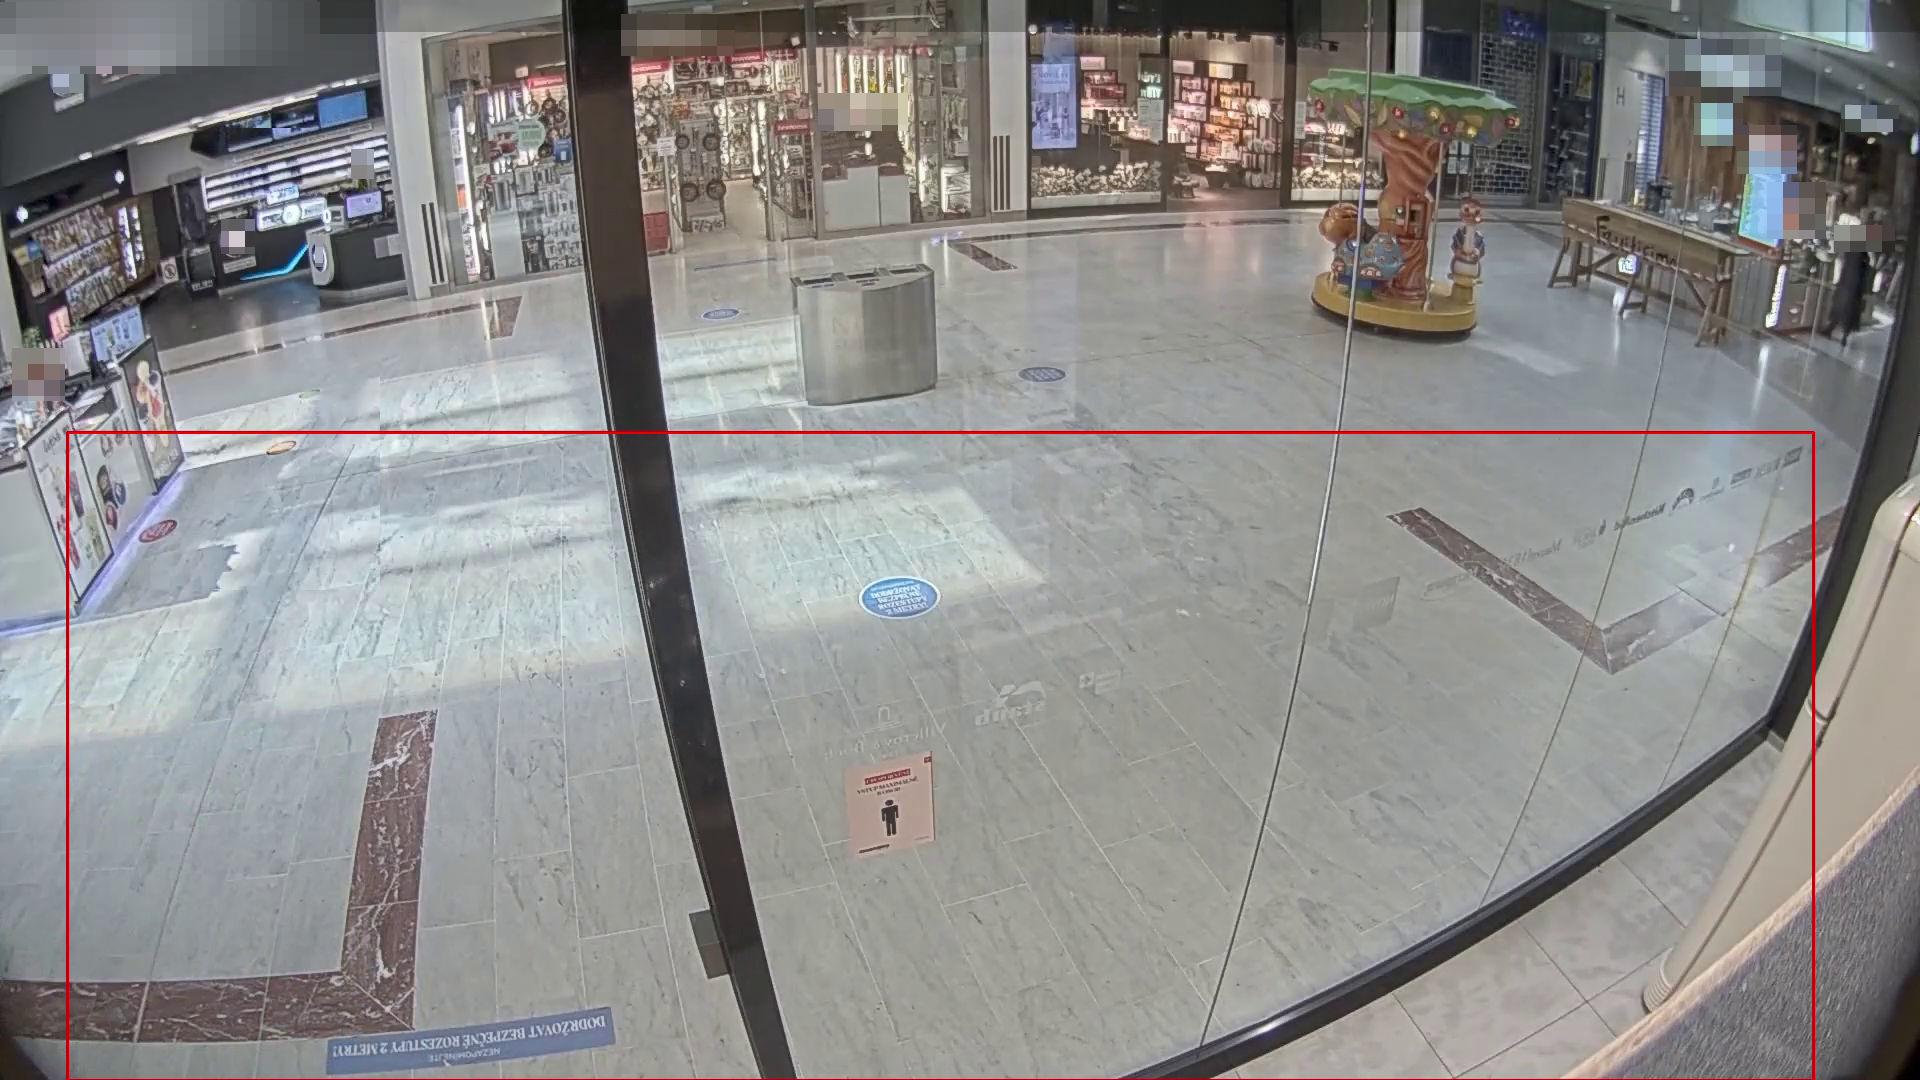
\includegraphics[width=8cm]{roi}
    \caption[A sample frame from the dataset with visualized \acrshort{roi}.]{A sample frame from the dataset with visualized \gls{roi}.}
    \label{fig:roi}
\end{figure}

We run the pipeline without the demographics extraction. We evaluate only tracks and annotations inside the \gls{roi}, a rectangle covering the relevant area in front of the shop. See figure \ref{fig:roi} for visualisation. Results are presented in table \ref{tab:tracker_results}. Final results are computed as an average of the evaluated sequences weighted by the number of frames. \textit{Switch ratio} is the ratio between the number of identity switches and the number of objects in total (scaled by 1000 for readability). We consider the minimal frame rate for real-time processing to be 10 \gls{fps}.

\textit{YOLOv4}\cite{bochkovskiy2020yolov4} is trained on the \textit{CrowdHuman}\cite{shao2018crowdhuman} dataset. \textit{PeopleNet}\cite{peoplenet} is trained on a proprietary NVIDIA dataset. The \textit{SSD}\cite{liu2016ssd} model is trained on the \textit{COCO}\cite{lin2014microsoft_coco} dataset and used with \textit{InceptionV2}\cite{ioffe2015batch_inception} as a feature extractor.

\begin{table}[hbt!]
    \centering
    \begin{tabular}{l|c|c|c|c}
        \hline
        Model & MOTA\,$\uparrow$ & MOTP\,$\uparrow$ & Switch Ratio\,$\downarrow$ & FPS\,$\uparrow$ \\
        \hline
        PeopleNet & 0.84 & 0.83 & \textbf{8.6} & 9.42 \\
        YOLOv4 & \textbf{0.91} & \textbf{0.93} & 8.7 & \textbf{13.0} \\
        SSD & 0.53 & 0.73 & 25 & 12.8
    \end{tabular}
    \caption{Tracker evaluation results with different detector models. The arrows indicate low or high optimal metric values.}
    \label{tab:tracker_results}
\end{table}

Based on the results, we selected the \textit{YOLOv4} model for use in the application. It has the best results in all categories except for the \textit{switch ratio}, where the results are very close to the best. Based on the metrics and visual evaluation of the algorithm's outputs, we consider its performance satisfactory.  We also consider the algorithm fast enough for real-time usage. 

Apart from our dataset, we also experimented on the MOT17\cite{MOT16} dataset, which is popular in literature. We have found the dataset to be too different from our target environment. The dataset contains videos taken from different angles and (often) with a moving camera. Our work assumes a stationary camera position at an elevated viewpoint, and so we have decided not to use the MOT17 dataset for evaluation. However, it remains an interesting source of data for testing the algorithm's robustness.

\section{Performance Optimization}

This section evaluates multiple architectures from a performance standpoint. In particular, we are interested in performance gain from using the TensorRT optimization framework.

We evaluate the \textit{SSRNet}\cite{yang2018ssr} and \textit{GoogLenet}\cite{szegedy2015going_googlenet} usable for age and gender classification. Further, we evaluate two \textit{OSNet}\cite{osnet} \gls{reid} architectures. As a baseline, we run the inference on CPU and GPU using \textit{ONNX Runtime}\cite{onnxruntime}, which is an open source machine learning framework. We then use the \textit{TensorRT} framework to optimize the model and run inference. The results are presented in table \ref{tab:cpu_gpu_trt}.

% ONNX runtime CPU, ONNX runtime GPU (CUDA), TensorRT (GPU - CUDA)
\begin{table}[hbt!]
    \centering
    \begin{tabular}{l|c|c|c}
        \hline
        Architecture & CPU & GPU & TensorRT \\
        \hline
        SSRNet (batch size 1) & 3.7 ms & 4.02 ms & 1.4 ms \\
        SSRNet (batch size 32) & 106 ms & 8.85 ms & 3.85 ms \\
        GoogLeNet & 144 ms & 12 ms & 3.17 ms \\
        \hline
        OSNet\_x0.25 & 361 ms & 41.8 ms & 12.3 ms \\
        OSNet\_ain\_x1.0 & 2.08 s & 156 ms & 53.8 ms
    \end{tabular}
    \caption{Inference time comparison.}
    \label{tab:cpu_gpu_trt}
\end{table}

We observe that using the \textit{TensorRT} optimized models increases performance about three times. To test that the optimization does not significantly decrease accuracy we evaluated the \textit{SSRNet} model on the \textit{MegaAge}\cite{huang2016unsupervised_megaage} dataset. The test \gls{mae} of the baseline version is  12.8, and the \gls{mae} of the optimized version is 14.4 (which is an error increase of 12.6\%).

Based on our experiments, we conclude that the \textit{TensorRT} framework can be used for significant performance gain while maintaining comparable results. However, it should be noted that the results may vary on different models or hardware.
